\section{Background on type qualifiers}
\label{sec:background}

\Cref{sec:must-call,sec:called-methods} describe
\emph{pluggable type systems}~\cite{FosterFFA99}
that are layered on top of the type system of the host
language.  Types in a pluggable type system are composed of two parts:
a \emph{type qualifier} and a base type. The type qualifier is the
part of the type that is unique to the pluggable type system; the base
type is a type from the host language. Our implementation is for Java
(see \cref{sec:implementation}), so we use the Java syntax for type
qualifiers: ``\<@>'' before a type indicates that it is a type
qualifier, and a type without ``\<@>'' is a base type.
This paper sometimes omits the basetype when it is obvious from context.

A type system checks programmer-written types.  Our system requires the
programmer to write types on method signatures, but within method bodies it
uses flow-sensitive type refinement, a dataflow analysis that performs type
inference.  This permits an expression to have different types on different
lines of the program.


% the technical sections about the core accumulation systems: called methods,
% must-call, and the must call invoked worklist algorithm.

\section{Cooperating analyses for leak detection}
\label{sec:base-type-systems}

This section presents a sound, modular, accumulation-based
resource leak checker.
\Cref{sec:lightweight-ownership,sec:reset-must-call,sec:must-call-choice}
enhance its precision.

\Tool is composed of three cooperating analyses:
\begin{enumerate}
\item a taint tracking type system (\cref{sec:must-call}) computes a conservative
  \emph{overapproximation} of the set of methods that might need to be called
  on each expression in the program.
\item an accumulation type system (\cref{sec:called-methods}) computes
  a conservative \emph{underapproximation} of the set of methods that are
  actually called on each expression in the program.
\item a dataflow analysis (\cref{sec:must-call-invoked}) computes, for
  every resource, a nonempty set of owning pointers.
  For each program point at which any owning pointer might go out of scope,
  it checks the consistency of the results of the two above-mentioned type systems.
  If any method that might need to be called is not in the set of methods
  that definitely were called, it issues an error.
\end{enumerate}

\begin{figure}
  \lstinputlisting{simplesocket.txt}
  \prefigcaption
  \caption{A safe use of a \<Socket> resource.}
  \label{fig:example}
\end{figure}

\noindent
This section uses \cref{fig:example} as a motivating example.
It shows
a safe use of a \<Socket>---a resource that must be closed before
it is deallocated.

\subsection{A type system for must-call obligations}
\label{sec:must-call}

\begin{figure}

\begin{tikzpicture}[->, shorten >= 1pt, auto, node distance=0.3cm]
  \tikzstyle{every state}=[fill=none,draw=none,text=black, minimum size = 0.5cm, shape = rectangle]
  
  \node[state]        (TOP)                                   {\parbox{4cm}  {\centering \small \<@MustCallUnknown> $= \top$}};
  \node[state]         (MCAB)      [below   = of TOP]        {\parbox{4cm}  {\centering \small \<@MustCall(\{"a", "b"\})>}};
  \node[state]         (MCA)    [below  = of MCAB, xshift=-2.2cm]         {\parbox{4cm} {\centering \small \<@MustCall(\{"a"\})>}};
  \node[state]         (MCB)    [below  = of MCAB, xshift=2.2cm]         {\parbox{4cm} {\centering \small \<@MustCall(\{"b"\})>}};
  \node[state]         (BOT)     [below      = of MCAB, yshift=-0.8cm]       {\parbox{4cm}  {\centering \small \<@MustCall(\{\})> $= \bot$}};

  \path

  (MCAB)        edge        node {} (TOP)
  
  (MCA)         edge        node {} (MCAB)
  (MCB)         edge        node {} (MCAB)
  
  (BOT)         edge        node {} (MCA)
  (BOT)         edge        node {} (MCB)

  ;

\end{tikzpicture}
% \prefigcaption
\caption{Part of the \<MustCall> type hierarchy for representing which methods must be
  called; the full hierarchy is a
  lattice of arbitrary size.
  If an expression's type has qualifier \<@Must\-Call(\{"a", "b"\})>, then
  the methods ``\<a>'' and ``\<b>'' might need to be called before the
  expression is deallocated.
  Arrows represent
  subtyping relationships.
}
\label{fig:must-call-hierarchy}
\end{figure}

The Must Call type system tracks
which methods might need to be called on
a given object before the object is deallocated.
This type system is general---it is not specific
to resource leaks.

The Must Call type system supports two qualifiers: \MustCall and
\MustCallUnknown. The \MustCall qualifier's arguments are the
methods that the annotated type must call. The declaration
\MustCall\<(\{"a"\}) Object obj> means that before \<obj> is
deallocated, \<obj.a()> might need to be called.
\Tool conservatively requires all these methods to be called,
and it issues a warning if they are not.

For example, consider \cref{fig:example}. The expression \<null> has type
\MustCall\<(\{\})>---it has no obligations
to call particular methods---so \<s> has that type after its initialization.
The \<new> expression has type \MustCall\<("close")>, and therefore
\<s> has that type after the assignment.
At the start of the \<finally> block, where both values for \<s> flow,
the type of \<s> is their least upper bound, which is \MustCall\<("close")>.

% Note that the type \MustCall\<("close")>
% can represent anything that \emph{might} need to
% call \<close()>: for example, at the entrance to
% the \<finally> block in \cref{fig:example}, \<s>'s
% actual value might either be \<null>, which does not
% need to call any methods, or an open \<Socket>, which does.
% Thus, either the obligation to close or no obligation at all
% can be represented by the static
% type \MustCall\<(\{"close"\}) Socket>, which can be read as ``a
% Socket that might need to call close before it is deallocated''.

Part of the type hierarchy appears in \cref{fig:must-call-hierarchy}.
All types are subtypes of \MustCallUnknown.
The subtyping relationship for \MustCall types is:
\trule{A \subseteq B}{\MustCall\<(A)> \sqsubseteq \MustCall\<(B)>}

The default type qualifier is \MustCall\<(\{\})> for base types without a
programmer-written type qualifier.\footnote{For unannotated local variable types,
  flow-sensitive type refinement infers a qualifier.}
% By writing another type qualifier on the declaration of a class, a
% user can specify a different default for raw types of that class.
Our implementation
provides JDK annotations which require that every 
\<Closeable> object must have the \<close()> method called before
it is deallocated.

% also provides an ``inheritable'' version of the \MustCall annotation,
% which allows us to annotate a class (or interface) and all of its subtypes.
% For example, we use such an annotation on \<java.io.Closeable> to indicate
% that all \<Closeable> objects must have the \<close()> method called before
% they are deallocated.

%% This is redundant, I think.
% A benefit of using a type system for tracking must-call obligations is
% that \Tool can use local type inference to refine the obligations of
% a particular variable. For example, if the only assignment to \<s>
% in \cref{fig:example} were the initial assignment to \<null>, then
% \Tool would be able to determine that \<s> does not have a must-call
% obligation.


\subsection{A type system for called methods}
\label{sec:called-methods}

% \todo{Mike changed ``our types system for inferring'' to ``our type system
%   tracks''.  Let's lay off use of ``infer'' because it implies we have
%   written a type inference tool, when what we have really written is a
%   type-checking tool (with local type inference).}

The Called Methods type system tracks a conservative underapproximation of which methods have been called on an object.
It is an extension of a similar system
from prior work~\cite{KelloggRSSE2020}.  The primary difference in our
version is that a method is considered called even if it throws an
exception---a necessity in Java because the \<close()> method
in \<java.io.Closeable> is specified to possibly throw an \<IOException>.
In the prior work, a method was only considered ``called'' when it terminated
successfully.
The remainder of this section is a brief summary
of the prior work~\cite{KelloggRSSE2020}.

% This checker is an \emph{accumulation analysis}: a special case
% of typestate analysis~\cite{StromY86} in which:
% \begin{enumerate}
% \item the order in which operations are performed cannot affect what is
%   subsequently permitted, and
% \item executing more operations does not add restrictions---that is,
%   the set of permitted operations after executing some operation is always
%   a superset of the set of permitted operations before executing that operation.
% \end{enumerate}
% This special case of typestate analysis is useful because it does not
% require a whole-program alias analysis for soundness, and instead
% can be implemented as a standard pluggable type system.

The checker is an accumulation analysis whose accumulation qualifier is \<@CalledMethods>.
The type \<@CalledMethods(>$A$\<) Object>
represents an object on which the methods in the set $A$ have definitely
been called; other methods not in $A$ might also have been called.
The subtyping
rule is:
\trule{B \subseteq A}{\<@CalledMethods(A)> \sqsubseteq \<@CalledMethods(B)>}
The top type is \<@CalledMethods(\{\})>.
The qualifier \CalledMethodsBottom is a subtype of every \<@CalledMethods> qualifier.

Thanks to flow-sensitive type refinement,
Called Methods types are inferred within method bodies.
In \cref{fig:example} the type of \<s> is initially \<@CalledMethods({})>,
but it transitions to \<@CalledMethods("close")> after the call to \<close>.


\subsection{Consistency checking}
\label{sec:must-call-invoked}

\begin{algorithm}[t]
  \caption{Finding unfulfilled \MustCall obligations in a method.
    \Cref{alg:helpers} defines helper functions.}
  \label{alg:consistency-checker}
  \begin{algorithmic}[1]
  \State \textit{// CFG represents a method}
  \Procedure{FindMissedCalls}{$CFG$}
  \State \textit{// D maps each statement s to a set of dataflow facts reaching}
  \State \textit{// s.  Each fact is of the form $\langle P, e \rangle$, where P is a set of variables}
  \State \textit{// that must-alias e and e is an expression with a nonempty}
  \State \textit{// must-call obligation.}
  \State $D \gets \textsc{InitialObligations}(CFG)$ \label{li:call-initial-obs}
  \While{$D$ has not reached fixed point}
    \For{$s \in \mathit{CFG.statements}$, $\langle P, e \rangle \in D(s)$}
    \If{$s$ is $\mathit{exit}$} \label{li:end-scope}
      \State report a must-call violation for $e$
    \ElsIf{$\neg \textsc{MCSatisfiedAfter}(P,s)$} \label{li:check-satisfied}
%    \State // \textit{propagate to successors}
    \State $kill \gets $ $s$ assigns a variable ? $\{s.LHS\}$ : $\emptyset$ \label{li:compute-kill}
    \State $gen \gets \textsc{CreatesAlias}(P,s)$ ? $\{s.LHS\}$ : $\emptyset$ \label{li:compute-gen} 
    % \If{$s$ is \lstinline{p = q} and $q \in P$}
    % \State $gen \gets \{p\}$
    % \EndIf
    \State $N \gets (P - kill) \cup gen$ \label{li:compute-new-mc-aliases}
 %   \State // \textit{we even propagate }$\emptyset$\textit{; error reported at exit}
    \State $\forall t \in \mathit{CFG.succ}(s)\ .\ D(t) \leftarrow D(t) \cup \langle
    N, e \rangle$ \label{li:prop-to-succs}
    \EndIf
    \EndFor
  \EndWhile \label{li:alg-loop-end}
  \EndProcedure
  \Procedure{InitialObligations}{$CFG$}
  \State $D \gets \{ s \mapsto \emptyset\ |\ s \in \mathit{CFG.statements} \}$\label{li:start-init}
  \For{$p \in \mathit{CFG.formals}$, $t \in \mathit{CFG.succ}(\mathit{CFG.entry})$}\label{li:init-formals}
    \If{$\textsc{HasObligation}(p)$}
      \State $D(t) \gets D(t) \cup \langle \{p\}, p \rangle$
    \EndIf
  \EndFor \label{li:end-init-formals}
  \For{$s \in \mathit{CFG.statements}$ of the form \lstinline{p = m(p1, p2, ...)}} \label{li:init-calls}
    \State $\forall t \in \mathit{CFG.succ}(s)\ .\ D(t) \leftarrow D(t) \cup \textsc{FactsFromCall}(s)$
  \EndFor  \label{li:end-init}
  \State \Return $D$
  \EndProcedure
  \end{algorithmic}
\end{algorithm}

\begin{algorithm}[h]
  \caption{Helper functions for \cref{alg:consistency-checker}.  Except for
  \textsc{MCAfter} and \textsc{CMAfter}, all functions will be replaced with
  more sophisticated versions in
  \cref{sec:lightweight-ownership,sec:must-call-choice,sec:reset-must-call}.
  \todo{Ensure the two algorithms appear on the same page.}
}
  \label{alg:helpers}
  \begin{algorithmic}[1]
  \State // \textit{Does e introduce a must-call obligation to check?}
  \Procedure{HasObligation}{$e$}
  \State \Return $e$ has a declared \MustCall type
  \EndProcedure
  \State // \textit{s must be a call statement p = m(p1, p2, ...)}
  \Procedure{FactsFromCall}{$s$}
  \State $p \gets s.LHS, c \gets s.RHS$
  \State \Return $\textsc{HasObligation}(c)$ ? $\{ \langle \{ p \}, c
  \rangle \}$ : $\emptyset$
  \EndProcedure
  \State // \textit{Is the must-call obligation for P satisfied after
    s?}
  \Procedure{MCSatisfiedAfter}{$P,s$}
  \State \Return $\exists p \in P .\ \textsc{MCAfter}(p,s) \subseteq \textsc{CMAfter}(p,s)$
  \EndProcedure
  \State // \textit{Does s introduce a must alias for a var in P?}
  \Procedure{CreatesAlias}{$P,s$}
    \State \Return $\exists \mathtt{q} \in P\ .\ s$ is of the form \texttt{p = q}
  \EndProcedure
  \Procedure{MCAfter}{$p,s$}
  \State \Return methods in \MustCall type of $p$ after $s$
  \EndProcedure
  \Procedure{CMAfter}{$p,s$}
  \State \Return methods in \<@CalledMethods> type of $p$ after $s$
  \EndProcedure
  \end{algorithmic}

\end{algorithm}

Given \MustCall and \<@CalledMethods> types, the Must
Call Consistency Checker ensures that \MustCall methods for each object
are always invoked before the object becomes unreachable.  This property is
checked via an intra-procedural dataflow analysis.  Here, we present
a simple, sound version of the analysis, with limited reasoning about aliasing.
\Cref{sec:lightweight-ownership,sec:must-call-choice,sec:reset-must-call}
describe enhancements to this basic approach.

\paragraph{Language} For simplicity, we present the analysis over a simple
assignment language in three-address form.  An expression $e$ in the language is
\<null>, a variable \<p>, a field read \<p.f>, or a method call \<m(p1,p2,\ldots)> (constructor
calls are treated as method calls).  A statement $s$ takes one of three forms:
\<p = e>, where $e$ is an expression; \<p.f = p'>, for a field write; or
\<return p>.  Methods are represented by a control-flow graph (CFG) where nodes
are statements and edges indicate possible control flow.  We elide control-flow
predicates as the consistency checker is path-insensitive.

% \manu{Martin, is the
% must-call checker path-sensitive?  As in, does it interpret null checks?}
% Martin's response: the Must Call Checker is path sensitive in the sense that
% it's flow sensitive and the type of null is bottom. It doesn't have any
% special logic to handle null checks, but it ``does the right thing''
% anyway.

For a method CFG, $\mathit{CFG.statements}$ is the statements,
$\mathit{CFG.formals}$ is the formal parameters,
$\mathit{CFG.entry}$ is its entry node,
$\mathit{CFG.exit}$ is its exit node, and
$\mathit{CFG.succ}$ is its successor relation.
For a statement
$s$ of the form \<p = e>, $s.LHS = p$ and $s.RHS = e$.

\paragraph{Pseudocode} \Cref{alg:consistency-checker} gives pseudocode for the
basic version of our checker, with helper functions in \cref{alg:helpers}.  At a
high level, the dataflow analysis computes a map $D$ from each statement $s$ in
a CFG to a \emph{set} of facts of the form $\langle P, e \rangle$, where $P$ is
a set of variables and $e$ is an expression.  The meaning
of $D$ is as follows: if $\langle P, e \rangle
\in D(s)$, then $e$ has a nonempty \MustCall type, and all variables in $P$
are \emph{must aliases} for the value of $e$ at the program point before $s$.
Computing a set of must aliases is useful since any must alias may be used to
satisfy the must-call obligation of $e$.  Using $D$, the analysis finds any $e$
that does not have its \MustCall obligation fulfilled, and reports an error.

\Cref{alg:consistency-checker} proceeds as follows.  \Cref{li:call-initial-obs}
invokes \textsc{InitialObligations} to initialize $D$.  Only formal parameters
or method calls can introduce obligations to be checked (not reads of local
variables or fields).
% \textsc{InitialObligations}
% (lines~\ref{li:start-init}--\ref{li:end-init}) scans for such expressions and
% adds initial facts as appropriate, using helper functions \textsc{HasObligation}
% and \textsc{FactsFromCall} from \cref{alg:helpers}.
The fixed-point loop
iterates over all facts $\langle P, e \rangle$ present in any
$D(s)$ (our implementation uses a worklist for efficiency).  If $s$ is the exit
node (\cref{li:end-scope}), the obligation for $e$ has not been satisfied, and
an error is reported.  Otherwise, the algorithm checks if the obligation for $e$
is satisfied after $s$ (\cref{li:check-satisfied}).  For the basic checker,
\textsc{MCSatisfiedAfter} in \cref{alg:helpers} checks whether there is some $p
\in P$ such that after $s$, the set of methods in $p$'s \MustCall type are contained
in the set of methods in its
\<@CalledMethods> type; if true, all \MustCall methods have already been
invoked.  This check uses the inferred flow-sensitive \MustCall and
\<@CalledMethods> qualifiers described in
\cref{sec:must-call,sec:called-methods}.
%% Mike doesn't see a way to resolve this comment.  Once MCAfter and
%% CMAfter are defined in the algorithm, that will tip off readers that
%% they are intended to be different and are not a typo.
% \todo{The names CMAfter and
% MCAfter are confusing - they're nearly identical. Can we think of better ones
% that are equally useful?} \manu{I don't have an idea that is also terse, but I
% am open to one.}

If the obligation for $e$ is not yet satisfied, the algorithm propagates the
fact to successors with an updated set $N$ of must aliases.  $N$ is computed in
a standard gen-kill style on
lines~\ref{li:compute-kill}--\ref{li:compute-new-mc-aliases}.  The kill set
simply consists of whatever variable (if any) appears on the left-hand side of
$s$.  The gen set is computed by checking if $s$ creates a new must alias for
some variable in $P$, using the \textsc{CreatesAlias} routine.  Since our
analysis is accumulation, \textsc{CreatesAlias} could simply return false
without impacting soundness.  In \cref{alg:helpers}, \textsc{CreatesAlias}
handles the case of a variable copy where the right-hand side is in $P$.
(\Cref{sec:must-call-choice} presents more sophisticated handling.) Finally,
\cref{li:prop-to-succs} propagates the new fact to successors.  The process
continues until $D$ reaches a fixed point.

\begin{figure}
  \begin{minipage}{0.4\columnwidth}
    \begin{lstlisting}
s = new Socket(...); // 1
if (...) {
  s = null; // 2
} else {
  t = s; // 3
  close(t); // 4
}
\end{lstlisting}
  \end{minipage}
  \begin{minipage}{0.55\columnwidth}
  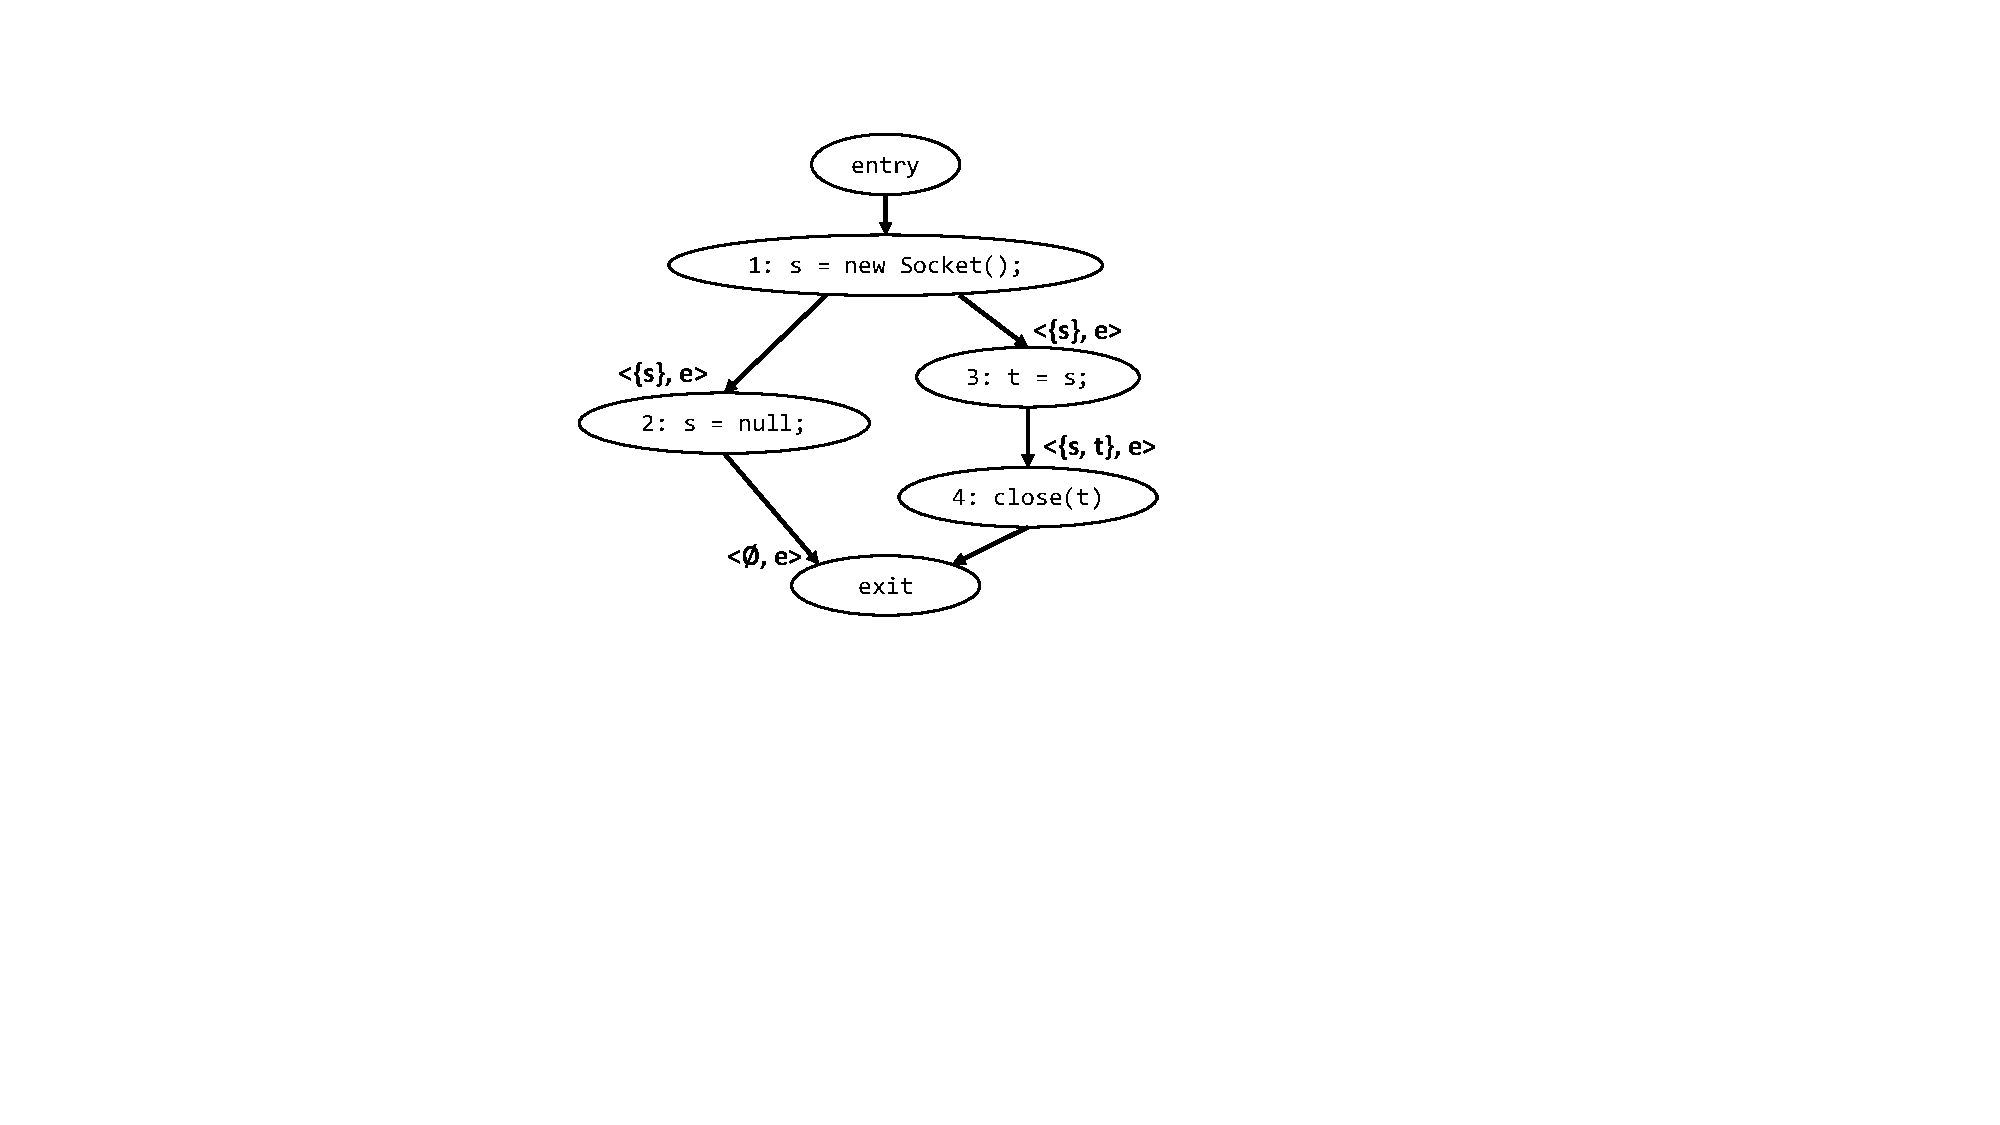
\includegraphics[width=\linewidth,keepaspectratio]{cfg-example.pdf}
  \end{minipage}
  \prefigcaption
  \caption{Example code and CFG for illustrating \cref{alg:consistency-checker}.
    ``\<e>'' is ``\<new Socket(...)>''.
} \label{fig:cfg-example}
\end{figure}

\paragraph{Example} To illustrate our analysis, \cref{fig:cfg-example} shows a
simple program (irrelevant details elided) and its corresponding CFG.
The CFG shows the dataflow facts propagated along each edge.
For initialization, statement 1 introduces the fact $\langle \{ s \}, e
\rangle$ (where $e$ is the \<new Socket(...)> call) to $D(2)$ and $D(3)$.  At
statement 2, $s$ is killed, causing $\langle \emptyset , e \rangle$ to be added
to $D(\mathit{exit})$.  This leads to an error being reported for statement 1, as
the socket is not closed on this path.  Statement 3 creates a must alias $t$ for
$s$, causing $\langle \{ s, t \}, e \rangle$ to be added to $D(4)$.  For
statement 4, $\textsc{MCSatisfiedAfter}(\{s,t\},\mathtt{close(t)})$ holds, so no
facts are propagated from 4 to $\mathit{exit}$.

At this point, we have described a sound checker for \MustCall obligations.
% But for real code, this checker emits too many false positives.  In particular,
% the dataflow analysis is purely intra-procedural, and it will report errors in
% cases where obligations are satisfied via parameter passing, returns, or fields.
Subsequent sections make the checker more precise.

% The Ownership Checker is a simple worklist algorithm that operates over the CFG.
% It maintains a set of owning pointers to objects, using a set of simple
% ownership rules:
% \begin{itemize}
% \item a newly-allocated object is owned
% \item the value returned by any method called is owned
% \end{itemize}

% These rules guarantee that there is at least one owning pointer to each
% object that might contain a resource. \Cref{sec:lightweight-ownership}
% gives more details on how ownership is transferred.

% When an owning pointer goes out of scope, the Ownership Checker
% compares the types computed by the Must Call Checker and the Called
% Methods Checker to determine if the requirements on the expression
% going out of scope have been fulfilled using the following process,
% supposing that some expression \<expr> is going out of scope at
% program point $P$:
% \begin{enumerate}
%   \item The Ownership Checker requests a Must Call type from the Must
%     Call Checker for \<expr> at $P$. Suppose this type is
%     \MustCall\<(>$A$\<)> for some set of methods $A$ (if the type is
%     \MustCallUnknown, the Ownership Checker always issues an
%     error).
%   \item The Ownership Checker requests a Called Methods type from the
%     Called Methods Checker for \<expr> at $P$. Suppose this type is
%     \<@CalledMethods(>$B$\<)> for some set of methods $B$.
%   \item The Ownership Checker compares the sets $A$ and $B$. If
%     $A \supset B$, the Ownership Checker issues an error.
% \end{enumerate}

% The Ownership Checker also does a simple, intra-procedural must-alias
% analysis, to avoid issuing duplicate errors for e.g. constructor
% invocations that are assigned to local variables. At most one error
% for each must-alias set is ever issued. 

% LocalWords:  simplesocket MustCallUnknown MCAB MustCall MCA xshift MCB
% LocalWords:  yshift Closeable CalledMethods CalledMethodsBottom IsExit
% LocalWords:  FindMissedCalls MCSatisfied CreatesAlias MCObligations p'
% LocalWords:  HasMCReturn EndOfScope CMBefore MCBefore basetype MCAfter
% LocalWords:  CMAfter HasObligation FactsFromCall MCSatisfiedAfter intra
% LocalWords:  InitialObligations worklist xleftmargin makeSocket addr
